% Celda de medición: corte lateral con sensores en la tapa (sin calc)
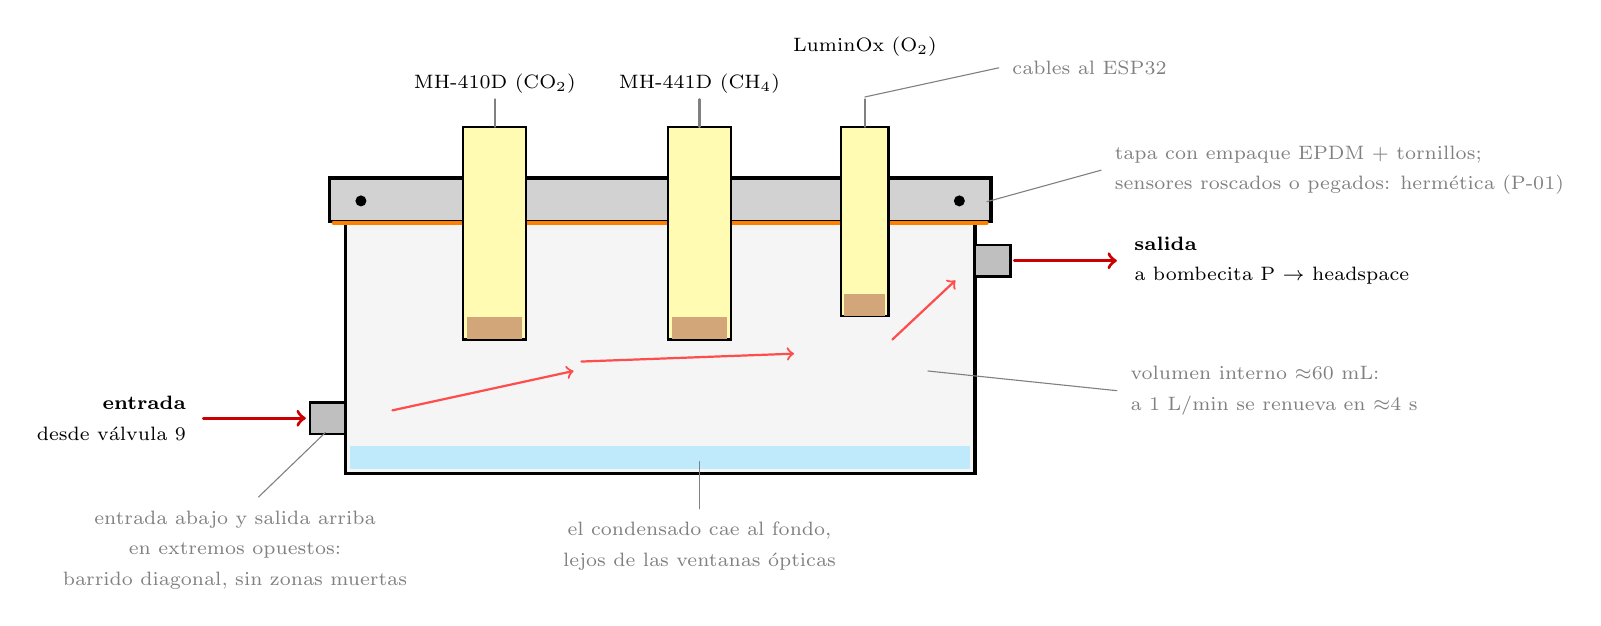
\begin{tikzpicture}[font=\small, line cap=round]

% --- cuerpo de la caja ---
\draw[very thick, fill=gray!8] (2.0,1.2) rectangle (10.0,4.4);
% condensado en el fondo
\fill[cyan!25] (2.06,1.26) rectangle (9.94,1.55);
% tapa con empaque
\draw[very thick, fill=gray!35] (1.8,4.4) rectangle (10.2,4.95);
\draw[orange, very thick] (1.85,4.38) -- (10.15,4.38);
\fill[black] (2.2,4.66) circle (0.07);
\fill[black] (9.8,4.66) circle (0.07);

% --- sensores en la tapa (cabezal hacia adentro y hacia abajo) ---
\draw[fill=yellow!30, thick] (3.5,2.9) rectangle (4.3,5.6);
\fill[brown!70] (3.55,2.9) rectangle (4.25,3.18);
\draw[fill=yellow!30, thick] (6.1,2.9) rectangle (6.9,5.6);
\fill[brown!70] (6.15,2.9) rectangle (6.85,3.18);
\draw[fill=yellow!30, thick] (8.3,3.2) rectangle (8.9,5.6);
\fill[brown!70] (8.34,3.2) rectangle (8.86,3.48);
% cables
\draw[thick, gray] (3.9,5.6) -- (3.9,5.95);
\draw[thick, gray] (6.5,5.6) -- (6.5,5.95);
\draw[thick, gray] (8.6,5.6) -- (8.6,5.95);
% nombres
\node at (3.9,6.15) {\scriptsize MH-410D (CO$_2$)};
\node at (6.5,6.15) {\scriptsize MH-441D (CH$_4$)};
\node at (8.6,6.62) {\scriptsize LuminOx (O$_2$)};
\draw[gray, thin] (8.6,5.98) -- (10.3,6.35);
\node[gray, anchor=west] at (10.35,6.35) {\scriptsize cables al ESP32};

% --- puertos ---
\draw[fill=gray!50, thick] (1.55,1.7) rectangle (2.0,2.1);
\draw[->, red!80!black, very thick] (0.2,1.9) -- (1.5,1.9);
\node[anchor=east, align=right] at (0.1,1.9) {\scriptsize \textbf{entrada}\\\scriptsize desde válvula 9};
\draw[fill=gray!50, thick] (10.0,3.7) rectangle (10.45,4.1);
\draw[->, red!80!black, very thick] (10.5,3.9) -- (11.8,3.9);
\node[anchor=west, align=left] at (11.9,3.9) {\scriptsize \textbf{salida}\\\scriptsize a bombecita P $\rightarrow$ headspace};

% --- barrido interno (por debajo de los cabezales) ---
\draw[->, red!70, thick] (2.6,2.0) -- (4.9,2.5);
\draw[->, red!70, thick] (5.0,2.62) -- (7.7,2.72);
\draw[->, red!70, thick] (8.95,2.9) -- (9.75,3.65);

% --- llamadas ---
\draw[gray, thin] (10.15,4.65) -- (11.6,5.05);
\node[gray, anchor=west, align=left] at (11.65,5.05)
  {\scriptsize tapa con empaque EPDM + tornillos;\\\scriptsize sensores roscados o pegados: hermética (P-01)};

\draw[gray, thin] (9.4,2.5) -- (11.8,2.25);
\node[gray, anchor=west, align=left] at (11.85,2.25)
  {\scriptsize volumen interno ${\approx}$60 mL:\\\scriptsize a 1 L/min se renueva en ${\approx}$4 s};

\draw[gray, thin] (6.5,1.35) -- (6.5,0.75);
\node[gray, anchor=north, align=center] at (6.5,0.7)
  {\scriptsize el condensado cae al fondo,\\\scriptsize lejos de las ventanas ópticas};

\draw[gray, thin] (1.75,1.72) -- (0.9,0.9);
\node[gray, anchor=north, align=center] at (0.6,0.85)
  {\scriptsize entrada abajo y salida arriba\\\scriptsize en extremos opuestos:\\\scriptsize barrido diagonal, sin zonas muertas};

\end{tikzpicture}
